% This is samplepaper.tex, a sample chapter demonstrating the
% LLNCS macro package for Springer Computer Science proceedings;
% Version 2.21 of 2022/01/12
%
\documentclass[runningheads]{llncs}
\usepackage{float}
\usepackage{pdfpages}
%
\usepackage[T1]{fontenc}
% T1 fonts will be used to generate the final print and online PDFs,
% so please use T1 fonts in your manuscript whenever possible.
% Other font encondings may result in incorrect characters.
%
\usepackage{graphicx}
% Used for displaying a sample figure. If possible, figure files should
% be included in EPS format.
%
% If you use the hyperref package, please uncomment the following two lines
% to display URLs in blue roman font according to Springer's eBook style:
\usepackage{hyperref}
\usepackage{color}
\renewcommand\UrlFont{\color{blue}\rmfamily}
\urlstyle{rm}
%
\begin{document}
%
\title{Fairness in Machine Learning Models (PER2024–030)}
\author{
    \textbf{Authors:} \\
    Adam Dienes \and 
    Bence Zsolt Beregi \\
    \textbf{Supervisors:} \\
    Mireille Blay-Fornarino \and 
    Anne-Marie Pinna-Dery \and 
    Nicolas Lacroix
}
\authorrunning{A. Dienes, B. Zs. Beregi }
% First names are abbreviated in the running head.
% If there are more than two authors, 'et al.' is used.
%
\institute{University Côte d'Azur, Campus SophiaTech, 930 route des Colles BP145, 06903 Sophia-Antipolis Cedex, France\\
\url{https://polytech.univ-cotedazur.fr} \\
\email{\{adam.dienes, bence-zsolt.beregi\}@etu.univ-cotedazur.fr} \\
\email{\{mireille.blay, anne-marie.pinna, nicolas.lacroix\}@univ-cotedazur.fr}
}
%
\maketitle              % typeset the header of the contribution
%
\begin{abstract}
As artificial intelligence increasingly influences critical decisions, ensuring model and dataset fairness is paramount. Our scientific research addresses the challenge of systematically visualizing and justifying the fairness of datasets and machine learning models throughout their lifecycle. We aim to bridge the gap between complex algorithms and real-world impact, empowering both model integrators and AI developers to build more equitable and transparent ML systems. We propose interactive visualizations that assess fairness without accessing sensitive attributes. Our approach integrates both pre-processing and post-processing techniques in ML to mitigate biases at multiple stages of the pipeline. 

\keywords{Machine Learning \and Model Fairness \and Dataset Fairness \and Interactive Visualization \and Bias Mitigation \and Transparency in AI \and Model Lifecycle \and Responsible AI \and Fairness Assessment Tools \and Bias Detection.}
\end{abstract}
%
%
%
\section{Introduction}
With the rise of Machine Learning (ML) models, it becomes crucial to ensure the fairness of these models throughout their lifecycle, leading states to propose frameworks to help organizations foster the responsible design, development, deployment and use of Artificial Intelligence (AI) systems over time. However, there is no systematic support to guide scientists and engineers in monitoring this property. This project aims to fill this gap by providing tools to visualize and justify the fairness of datasets and ML models.

\section{Description}
As ML models increasingly influence important choices in industries like recruiting, finance, healthcare and law enforcement, there is rising concern about ensuring justice in these algorithms. Unfair results can arise from biases in (historical) data or model behavior which disproportionately affect particular demographic groups. Even though fairness is acknowledged to be important, there are still insufficient systematic tools and procedures to track and support fairness across the whole lifecycle of datasets and models.\\

Large datasets and complicated systems may not be adequately served by the post-analysis and manual inspection methods that are frequently used in current fairness auditing techniques. Furthermore, access to sensitive characteristics like socioeconomic status, gender or ethnicity is necessary for many fairness evaluation techniques. Due to the lack of such data, this raises privacy and bias issues.\\

Furthermore, it can be difficult for AI engineers and even for model integrators to connect technical fairness metrics with practical applications and actionable recommendations. For non-experts, it can be quite challenging to understand at first sight and convert current fairness measurements into useful information. These difficulties are made worse by the lack of user-friendly, interactive visualization tools. It is challenging to identify problems and compare models or perform fairness assessments to larger audiences in the absence of unmistakable, visual representations.\\

This research focuses on addressing these gaps by developing interactive visual tools to assess fairness without relying on sensitive attributes. This tool aims to detect and mitigate bias while promoting transparency, recommendation and most importantly understanding. 

\section{State-of-the-art}
Fairness and bias prevention in machine learning have emerged as essential research fields as AI systems are being used in high-impact domains such as healthcare, recruitment, lending and criminal justice. Despite their strength, these systems frequently reinforce or inherit prejudices from their data or algorithms, which raise moral, societal and legal issues. While adherence to this property is crucial, evaluating the fairness of a system incorporating a ML model remains challenging. This is because the understanding of fairness varies across different contexts. This summary of the state-of-the-art explores the latest approaches, challenges and resources for addressing biases and advancing fairness in machine learning. The review aims to identify the key conceptual and visual elements necessary to characterize and promote the evaluation and justification of "fairness".

\subsection{Challenges in Achieving Fairness}
The difficulty of defining fairness is one of its greatest obstacles. Different ethical concerns are reflected in the various formal definitions of fairness\cite{precioso2024ethical}, including equality of odds, statistical parity/demographic parity, equal opportunity, disparate/adverse impact, PPV-parity, FPR-parity and NPV-parity ~\cite{fraenkel2020fairness}. These definitions, however, frequently clash, making it impossible to accomplish them all at once. The impossibility theorem, which illustrates the intrinsic trade-offs among fairness criteria, effectively captures the difficulties of balancing fairness standards in machine learning ~\cite{bell2023fairness}.\\

For instance, when base rates vary between groups, it is theoretically difficult to achieve "predictive parity" (equalizing positive predictive value across groups) and "classification parity" (equalizing false positive and false negative rates). This suggests that, depending on the criteria given priority, fairness interventions invariably jeopardize other goals, such as overall accuracy or equitable error rates  ~\cite{dibello2021fairness,nguyen2022fairness}.\\

Similarly, the impossible finding by Kleinberg et al. ~\cite{kleinberg2016} demonstrates that when base rates differ, goals such as classification balance (equal average risk scores for positives and negatives across groups) and predictive calibration (uniform interpretation of risk scores across groups) cannot co-exist. This emphasizes how fairness modifications frequently call for sacrificing accuracy or giving preference to one fairness metric over another.\\

As demonstrated by tools such as \href{https://en.wikipedia.org/wiki/COMPAS_(software)}{COMPAS software}, where balancing fairness metrics resulted in differences in false positive and false negative rates between demographic groups, these trade-offs call into question the practical usefulness of fairness modifications. ~\cite{yap2024} Another significant issue is bias in training data. Historical injustices, institutionalized prejudice, or the underrepresentation of particular groups are frequently reflected in data. Therefore, discriminatory results can be obtained from even seemingly "unbiased" models. Effectively diagnosing and mitigating bias is further complicated by intersectionality, which is the combined influence of several protected characteristics (such as race, religion, gender, sexual orientation and ethnicity).\\

In essence, achieving fairness in ML is a multifaceted challenge that necessitates a deliberate examination of the context, objectives and definitions applied. As Bell et al.~\cite{bell2023fairness} highlight, fairness often involves unavoidable trade-offs between competing goals and acceptable error levels. By surfacing and explicitly addressing these compromises, practitioners can better navigate the intricate interplay of factors such as bias, intersectionality and contextual nuances. This approach fosters transparency and accountability, paving the way toward models that more effectively balance fairness and utility in real-world applications.

\subsection{Fairness and Bias Mitigation Techniques}
Pre-processing, in-processing and post-processing strategies are the three main categories into which efforts to reduce bias in machine learning models fall ~\cite{prince2019}.\\

The goal of pre-processing techniques (agnostic to ML approach) is to lessen bias in the input of data prior to training. While reweighing approaches give training samples various weights depending on their representation, techniques such as disparate impact reduction modify feature distributions to lessen discrepancies between groups. By using causal inference to detect and address biases resulting from protected features, causal fairness approaches go one step further. There are additional techniques as well like massaging the data, sampling and correlation remover.\\

To apply fairness restrictions during model training, in-processing techniques step in (modification of the algorithm to remove discrimination). One popular technique is adversarial de-biasing, which uses a two-part model in which the primary predictor reduces the adversary's capacity to identify protected features. By incorporating fairness penalties into the model's loss function, fair regularization makes sure the model optimizes for both accuracy and fairness. Fairness restrictions are especially incorporated into the topologies of some neural networks. ~\cite{voria2024}\\

\begin{figure}
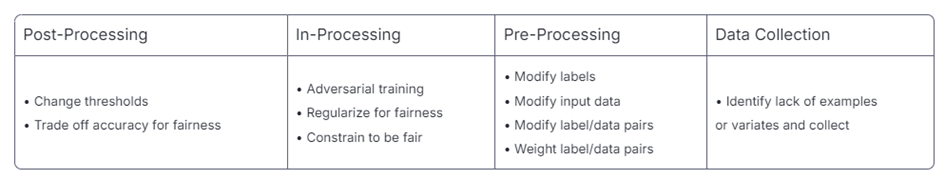
\includegraphics[width=\textwidth]{images/categories.png}
\caption{The main categories of reducing bias / Source: www.rbcborealis.com} \label{categories}
\end{figure}

After training, post-processing methods adjust model predictions to attain fairness. Predictions are adjusted using techniques like equalized odds post-processing to balance error rates (such as false positives and true positives) among groups. To reduce inequities, threshold modifications use distinct judgment thresholds for various groups.\\

The alignment between the fairness definition and the chosen technique ensures that the objectives are not only met but also appropriately justified within the given context. Therefore, it is essential to select a method that both promotes fairness in line with the definition being applied and effectively communicates the rationale behind its use ~\cite{hardt2016}.

\subsection{Metrics for Measuring Fairness}
Metrics that measure bias at the individual and group levels are essential to the assessment of fairness. While equalized odds assess consistency in true and false positive rates, group fairness criteria like statistical parity gauge how consistently positive results occur across groups. \\

Disparate impact, which is frequently employed in regulatory situations, measures the proportion of favorable outcomes between groups. Metrics of individual fairness evaluate whether the model predicts similar outcomes for similar people. Trade-off measures, which frequently strike a balance between justice and accuracy or other performance goals, quantify how fairness interventions affect utility. However, despite the availability of these metrics, there are still significant gaps in the ability to easily assess and justify the fairness of a model. Many of these indicators are complex and require specialized knowledge to interpret correctly. More thorough visualizations that can incorporate numerous indications and offer a comprehensive perspective of a model's fairness are also required ~\cite{bengio2024}.

\subsection{Tools and Frameworks for Fairness}
Several open-source tools have been created to help practitioners assess and reduce prejudice. A comprehensive collection of fairness metrics and mitigation strategies is offered by IBM's \href{https://aif360.res.ibm.com/}{AI Fairness 360} (AIF360). \href{https://themis-ml.readthedocs.io/en/latest/}{Themis-ML} specializes in bias detection and fairness-aware machine learning, while \href{https://fairlearn.org/}{Fairlearn} concentrates on Python-based fairness evaluation and mitigation. By providing an interactive interface for investigating fairness in machine learning models, \href{https://pair-code.github.io/what-if-tool/}{Google's What-If Tool} helps practitioners see and comprehend the effects of changes.

\begin{figure}
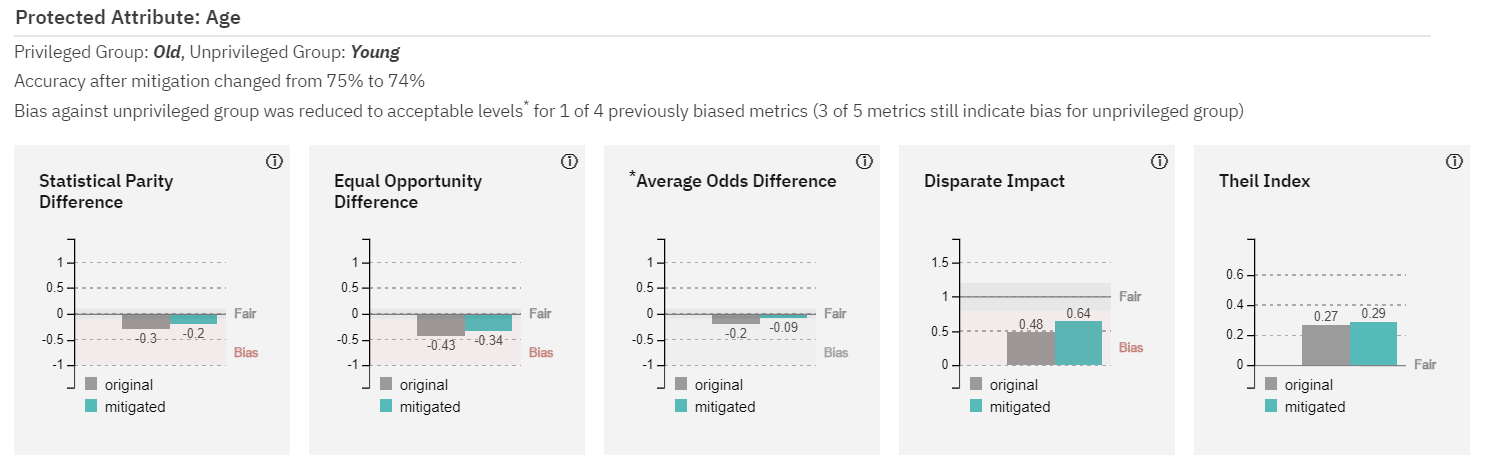
\includegraphics[width=\textwidth]{images/aif360.png}
\caption{AIF360 metrics dashboard / Source: aif360.res.ibm.com} \label{aif360}
\end{figure}

At first look, it can be difficult to understand fairness metric representations in ML and it frequently takes a lot of work to rigorously evaluate and implement insights. Even if existing tools like bias heatmaps, disparity matrices and fairness dashboards offer helpful visualizations of bias and fairness indicators, there is still much space for improvement in terms of their usability and accessibility ~\cite{mbakwe2023}.\\

For instance, users can interactively compare measures like equalized chances and demographic parity using fairness dashboards like Fairlearn and AIF360. However, consumers without a strong technical background may find these visualizations too comprehensive. Despite their visual compactness, bias heatmaps and disparity matrices frequently need to be carefully interpreted in order to understand subtle intersectional biases or fairness breaches ~\cite{zohar2023}.\\

Integrating explainability tools (e.g. \href{https://shap.readthedocs.io/en/latest/}{SHAP}) into these visualizations is a step forward but can add additional layers of complexity. For non-expert users, even sophisticated techniques like dimensionality reduction (e.g. t-SNE) to visualize biases in data clusters are not intuitive by nature. A recurring issue is the absence of tools designed to foster intuitive understanding rather than relying solely on mathematical representations. For instance, Chouldechova \cite{chouldechova2017} points out that although fairness-related proofs could be succinct, their dependence on technical terms and mathematical jargon rather than visual or descriptive methods sometimes prevents them from evoking perception. This highlights a crucial need: the requirement for tools that bridge the gap between intricate technical principles and practical understanding through understandable, interactive representations and examples. The possibility of combining visual aids with real-world examples to make fairness metrics easier to comprehend and apply.\\

Even with continuous advancements, the needs of various stakeholders—from business executives to legislators—cannot be adequately met by the visual techniques currently in use. To overcome these limitations and allow both technical and non-technical users (model integrators) to participate meaningfully with fairness-related concerns in machine learning, more interactive, intuitive and instructional visualization techniques are needed.

\subsection{Recent Advances in Fairness}
Integrating fairness with innovative technology and approaches has been the focus of recent study. For example, causal inference is used in causal fairness techniques to separate the effects of protected traits from the actual causes of outcomes. To guarantee that predictions stay fair in the face of such changes, counterfactual fairness techniques investigate how modifications to sensitive qualities affect model predictions. With multi-adversary systems addressing fairness across several protected qualities at once, adversarial learning remains a thriving area of innovation. Fairness-aware \href{https://www.automl.org/automl/}{AutoML}, in which automated machine learning algorithms integrate fairness restrictions into the optimization process, is another noteworthy trend.

\subsection{Future Directions and Summary}
Hybrid approaches that include pre-, in- and post-processing techniques are becoming more and more popular as fairness research progresses. These methods promise to address issues of justice in a more comprehensive way. Furthermore, because they facilitate accurate diagnosis and effective communication of bias-related problems, interpretability and explainability are increasingly becoming crucial elements of fairness research.\cite{google2024bias}\\

However, the creation of better visualization methods—tools that are user-friendly and efficient in conveying insights linked to fairness—is one of the most urgent demands. The field can close the gap between technical complexity and practical understanding by concentrating on developing more approachable, interactive and example-driven visualization techniques, guaranteeing that fairness becomes an understandable and achievable objective for all parties involved.

\section{Methodology}
As noted in our state-of-the-art review, our study methodology is designed to tackle the difficulties associated with fairness assessment in machine learning with a specific emphasis on the need for more interactive, intuitive and educational visualization tools. In keeping with the recognized need for instruments that close the gap between complex technical concepts and real-world knowledge, our strategy combines the creation of a new software tool with a thorough assessment methodology.

\subsection{Tool Development}
We adopted an iterative, user-centered design process for developing our fairness assessment tool, leveraging the strengths of \href{https://jupyter.org}{Jupyter Notebook} for rapid prototyping and Mercury for creating a user-friendly interactive front-end. The initial phase involved a comprehensive requirements-gathering process, identifying key needs based on challenges and gaps documented in current research. These requirements included support for a variety of fairness metrics – Statistical Parity/Demographic Parity, Equality of Odds, Equal Opportunity, Disparate Impact and MinDiff – accompanied by intuitive visualizations capable of conveying the meaning and implications of these metrics to both technical and non-technical users. Further requirements included actionable guidance for mitigating fairness issues and a mechanism for justifying interventions and documenting trade-offs. Prototyping initial versions of the tool in Jupyter Notebook then emphasized core functionalities like data upload, attribute selection, metric calculation and visualization.\\

This was followed by actively soliciting feedback from a diverse group of potential users, including machine learning practitioners, domain experts and individuals with limited technical expertise, to refine the tool's design, enhance its usability and ensure that it effectively met the needs of its target audience. Based on this user feedback, the final implementation incorporated key features such as a user-friendly interface for CSV dataset upload, automated calculation of fairness metrics, interactive visualizations tailored to each metric, contextual guidance for addressing fairness issues and a justification module for documenting interventions.\\\\ Our technology stack consists of  \href{https://www.python.org}{Python}, \href{https://jupyter.org}{Jupyter Notebook}, \href{https://runmercury.com}{Mercury}, \href{https://pandas.pydata.org}{Pandas}, \href{https://scikit-learn.org/stable}{Scikit-learn}, \href{https://plotly.com/python}{Plotly} and \href{https://matplotlib.org}{Matplotlib}.

\begin{figure}
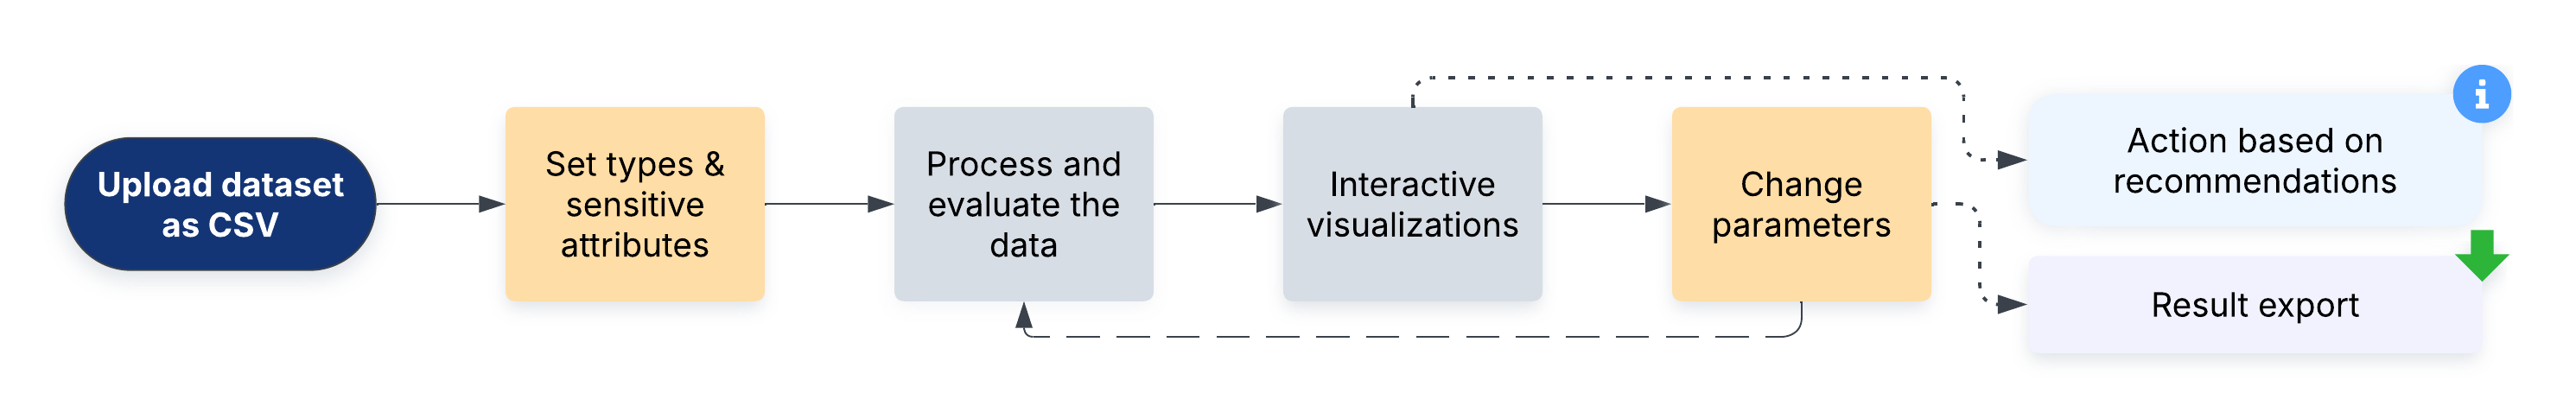
\includegraphics[width=\textwidth]{images/workflow.png}
\caption{Workflow of the application} \label{workflow}
\end{figure}

\subsection{Evaluation Framework}

\subsection{Experimental Procedure and Ethical Considerations}
Our experimental procedure involved a carefully controlled process consisting of a baseline experiment, an intervention experiment and a detailed comparison. During the baseline experiment, machine learning models were trained on the selected datasets without using our tool, thus establishing a control for assessing any improvements achieved through intervention. Subsequently, in the intervention experiment, users were provided with our tool and asked to identify and mitigate fairness issues, allowing us to observe how effectively the tool facilitated these actions. A final comparison then assessed the impact of our tool on fairness. In all aspects of our research, we adhered to strict ethical guidelines. The collected data was anonymized. By following this methodology, we aim to demonstrate the effectiveness of our fairness assessment tool in empowering users to build more equitable and transparent AI systems.

\section{Solution}
Our research introduces a novel software tool designed to empower users to detect, visualize and address fairness issues within their datasets and machine-learning models. Developed using Jupyter Notebook and leveraging the interactive capabilities of Mercury for a user-friendly front-end, our solution allows users to effortlessly upload CSV datasets and designate numeric, categorical, sensitive and prediction attributes. This streamlined process forms the foundation for a comprehensive fairness analysis and model training workflow.\\

\begin{figure}
\centering
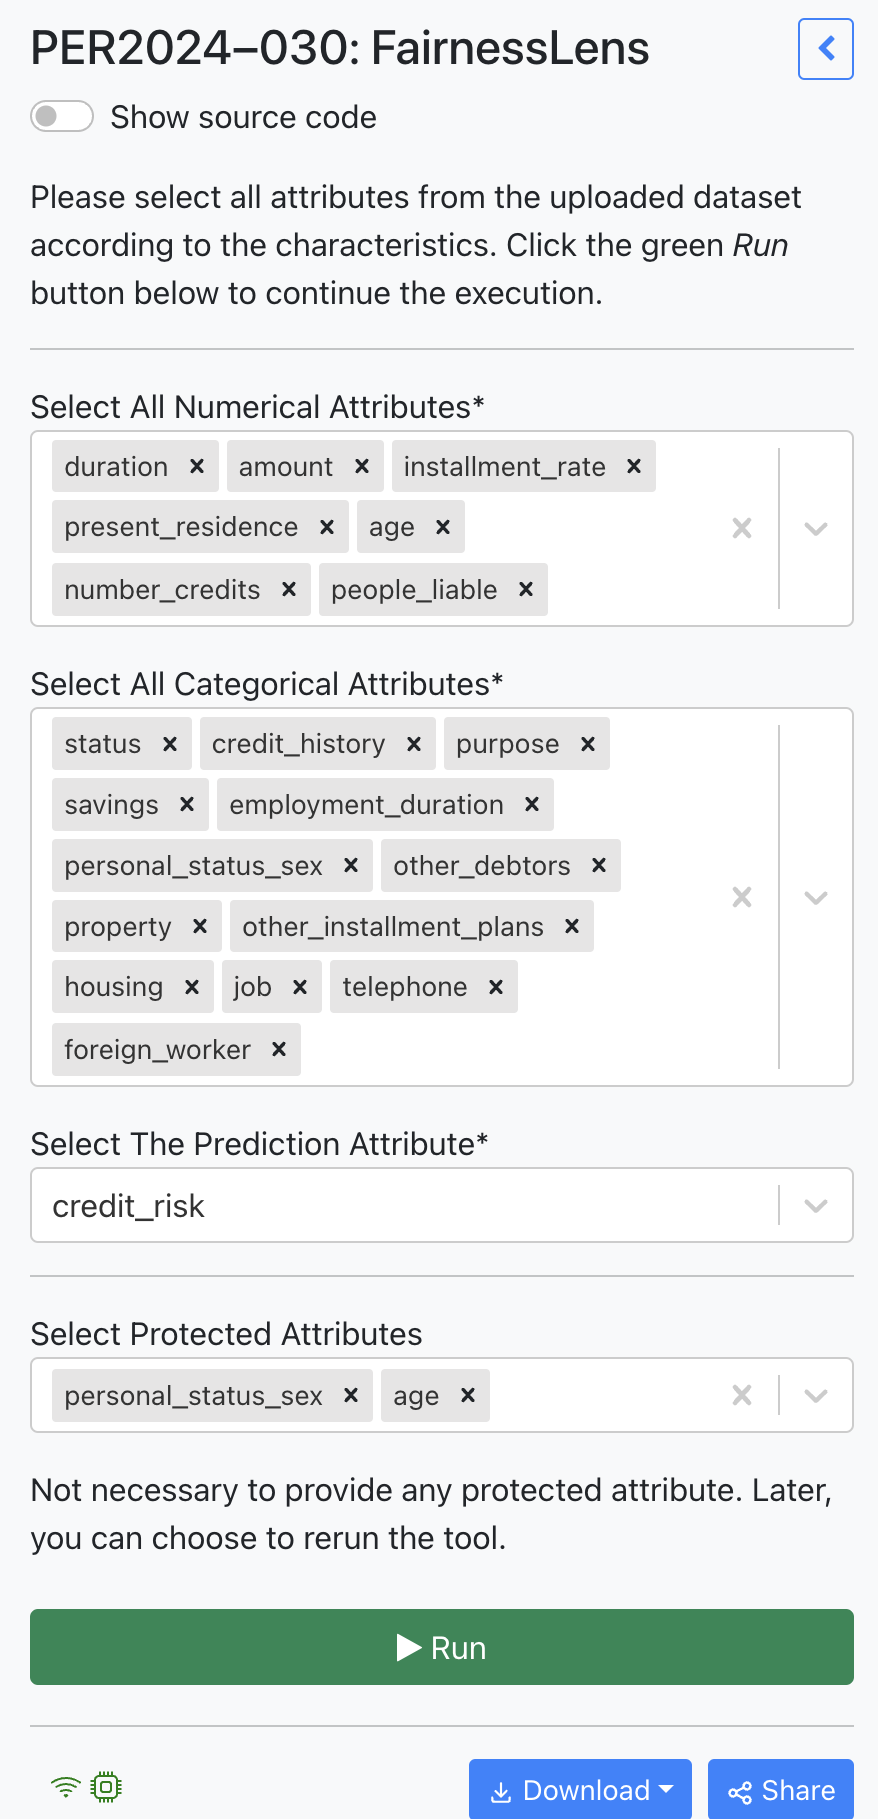
\includegraphics[width=0.3\textwidth]{images/mercury-interface.png}
\caption{Mercury frontend interface} \label{}
\end{figure}

The core of our solution lies in its ability to analyze several key fairness metrics, providing insightful details and actionable guidance based on the results. By offering a combination of metric evaluation, visualization and recommendations, we aim to bridge the gap between complex algorithmic concepts and practical implementation, making fairness assessment accessible to both technical and non-technical users.

\begin{figure}[H]
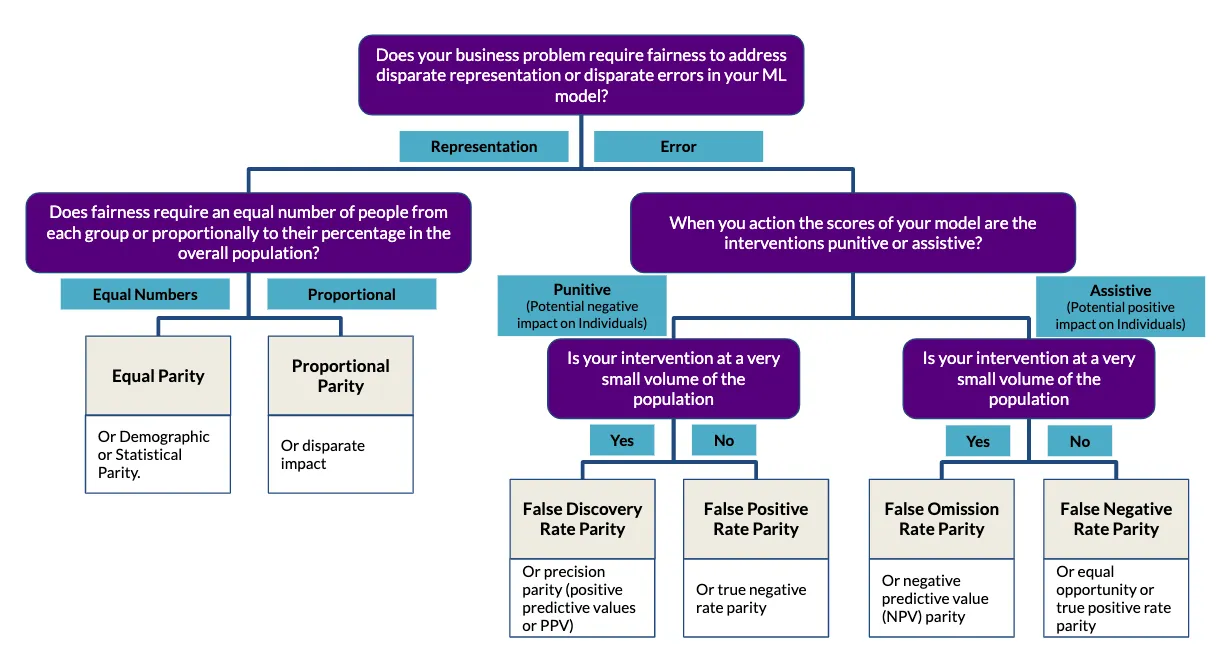
\includegraphics[width=\textwidth]{images/fairness-tree.png}
\caption{The Fairness Tree / Source: http://www.datasciencepublicpolicy.org/projects/aequitas} \label{fairness-tree}
\end{figure}

The key metrics we analyze include:

\subsection{Statistical Parity / Demographic Parity}
Also known as "group fairness," Demographic Parity (DP) aims to ensure that the likelihood of receiving a positive outcome from a model is the same across all groups, regardless of their protected attribute (e.g., gender, race, age). This means the model's decisions should not be influenced by sensitive characteristics, leading to equal representation in positive outcomes across different groups.

\begin{equation}
P(\hat{y} = 1 \mid p=0) = P(\hat{y} = 1 \mid p=1)
\end{equation}
Where:
\begin{itemize}
    \item $\hat{y}$ represents the predicted outcome.
    \item $p$ represents the protected attribute.
\end{itemize}

In simpler terms, if a model predicts loan approvals, Demographic Parity would mean that the proportion of loan approvals should be roughly the same for men and women. A violation of DP suggests the model might be discriminating, even if unintentionally.\\

Our tool uses bar charts to illustrate this. Each bar represents a protected attribute and the width of the bar shows the proportion of DP difference from an optimal value of 0. If the bar is significantly wide, it is displayed with red color and indicates a potential DP violation (favors privileged). This straightforward visual representation helps users quickly identify whether positive outcomes are evenly distributed across groups.

\begin{figure}
\centering
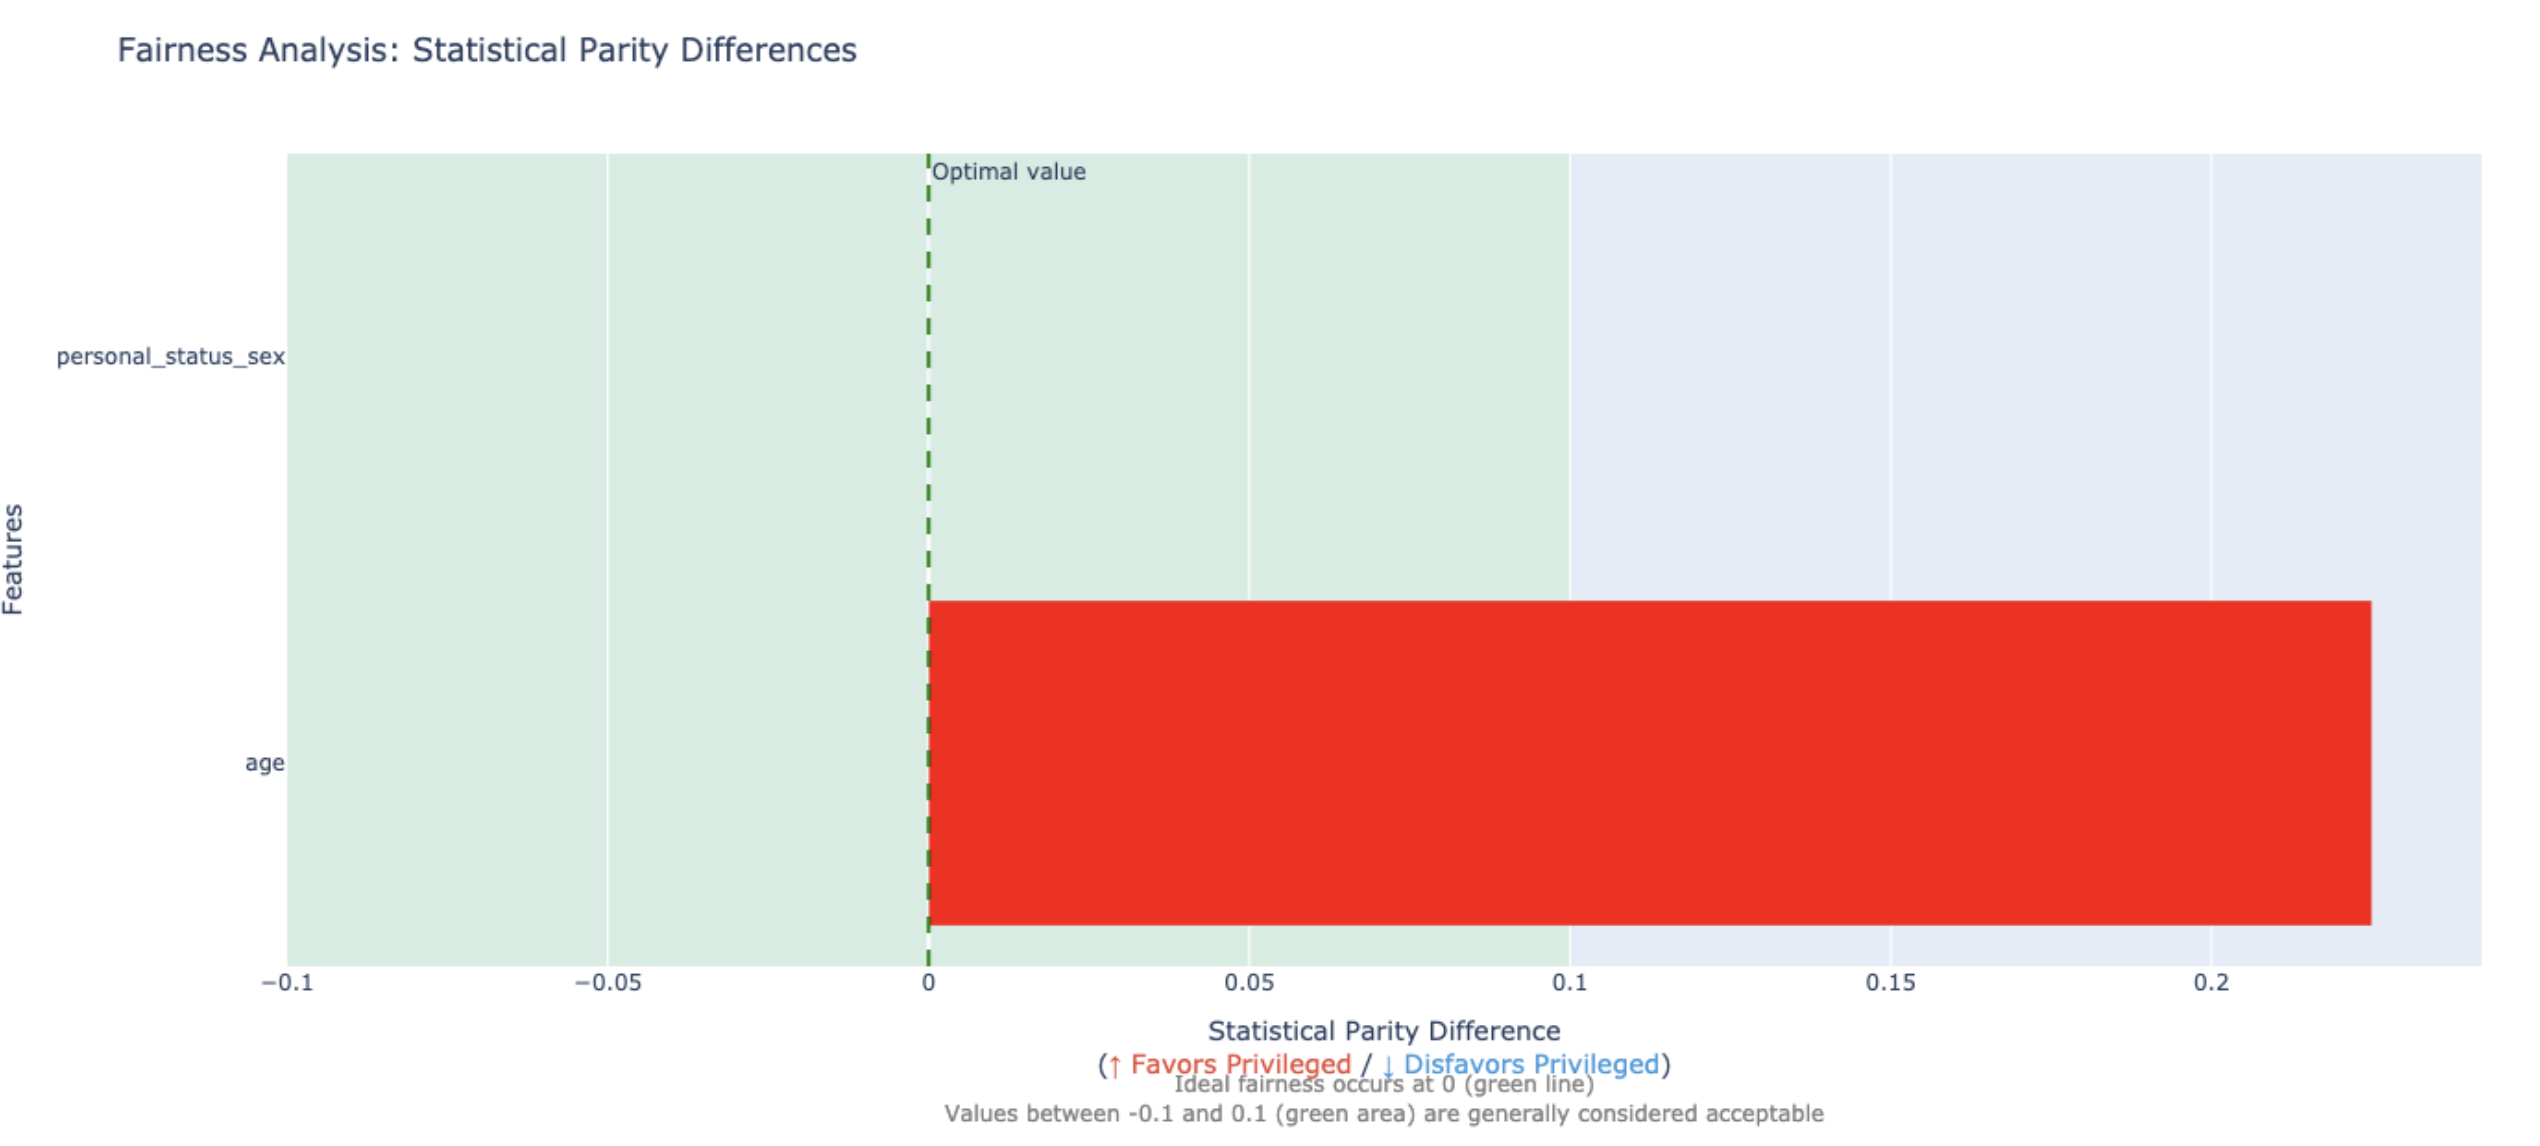
\includegraphics[width=1\textwidth]{images/sp-chart.png}
\caption{Demographic / Statistical Parity chart} \label{sp-chart}
\end{figure}

\subsection{Equality of Odds and Equal Opportunity}
Equality of Odds seeks to ensure that the model performs equally well for all groups, considering both the True Positive Rate (TPR) and the False Positive Rate (FPR). In essence, the model should have similar accuracy and error rates across different groups. This implies conditional independence of the predicted outcome and the protected attribute given the true outcome. \\

Regardless of whether they belong to a protected group, those who are eligible for a favorable outcome (such as loan approval, job hiring or college admission) are treated equitably thanks to the equal opportunity criterion. In particular, the TPR must be the same for all groups for Equal Opportunity to be met. This implies that the protected property shouldn't affect the likelihood of obtaining a good outcome among individuals who actually qualify for one (i.e., where y=1).

\begin{equation} 
P(\hat{y} = 1 | p=0, y=1) = P(\hat{y} = 1 | p=1, y=1) 
\end{equation}

Equal Opportunity is just concerned with making sure that eligible people are not disadvantaged because they belong to a certain group, as opposed to Equality of Odds, which also takes FPR into account. This is especially crucial in situations where equity in favorable results is a top concern, such as recruiting, lending and medical diagnosis.\\

We visualize this using grouped bar charts with True/False Positive/Negative rates across all selected protected attributes. This allows users to quickly compare these values for each attribute and identify any significant disparities, which would indicate a potential violation of equal opportunity.

\begin{figure}
\centering
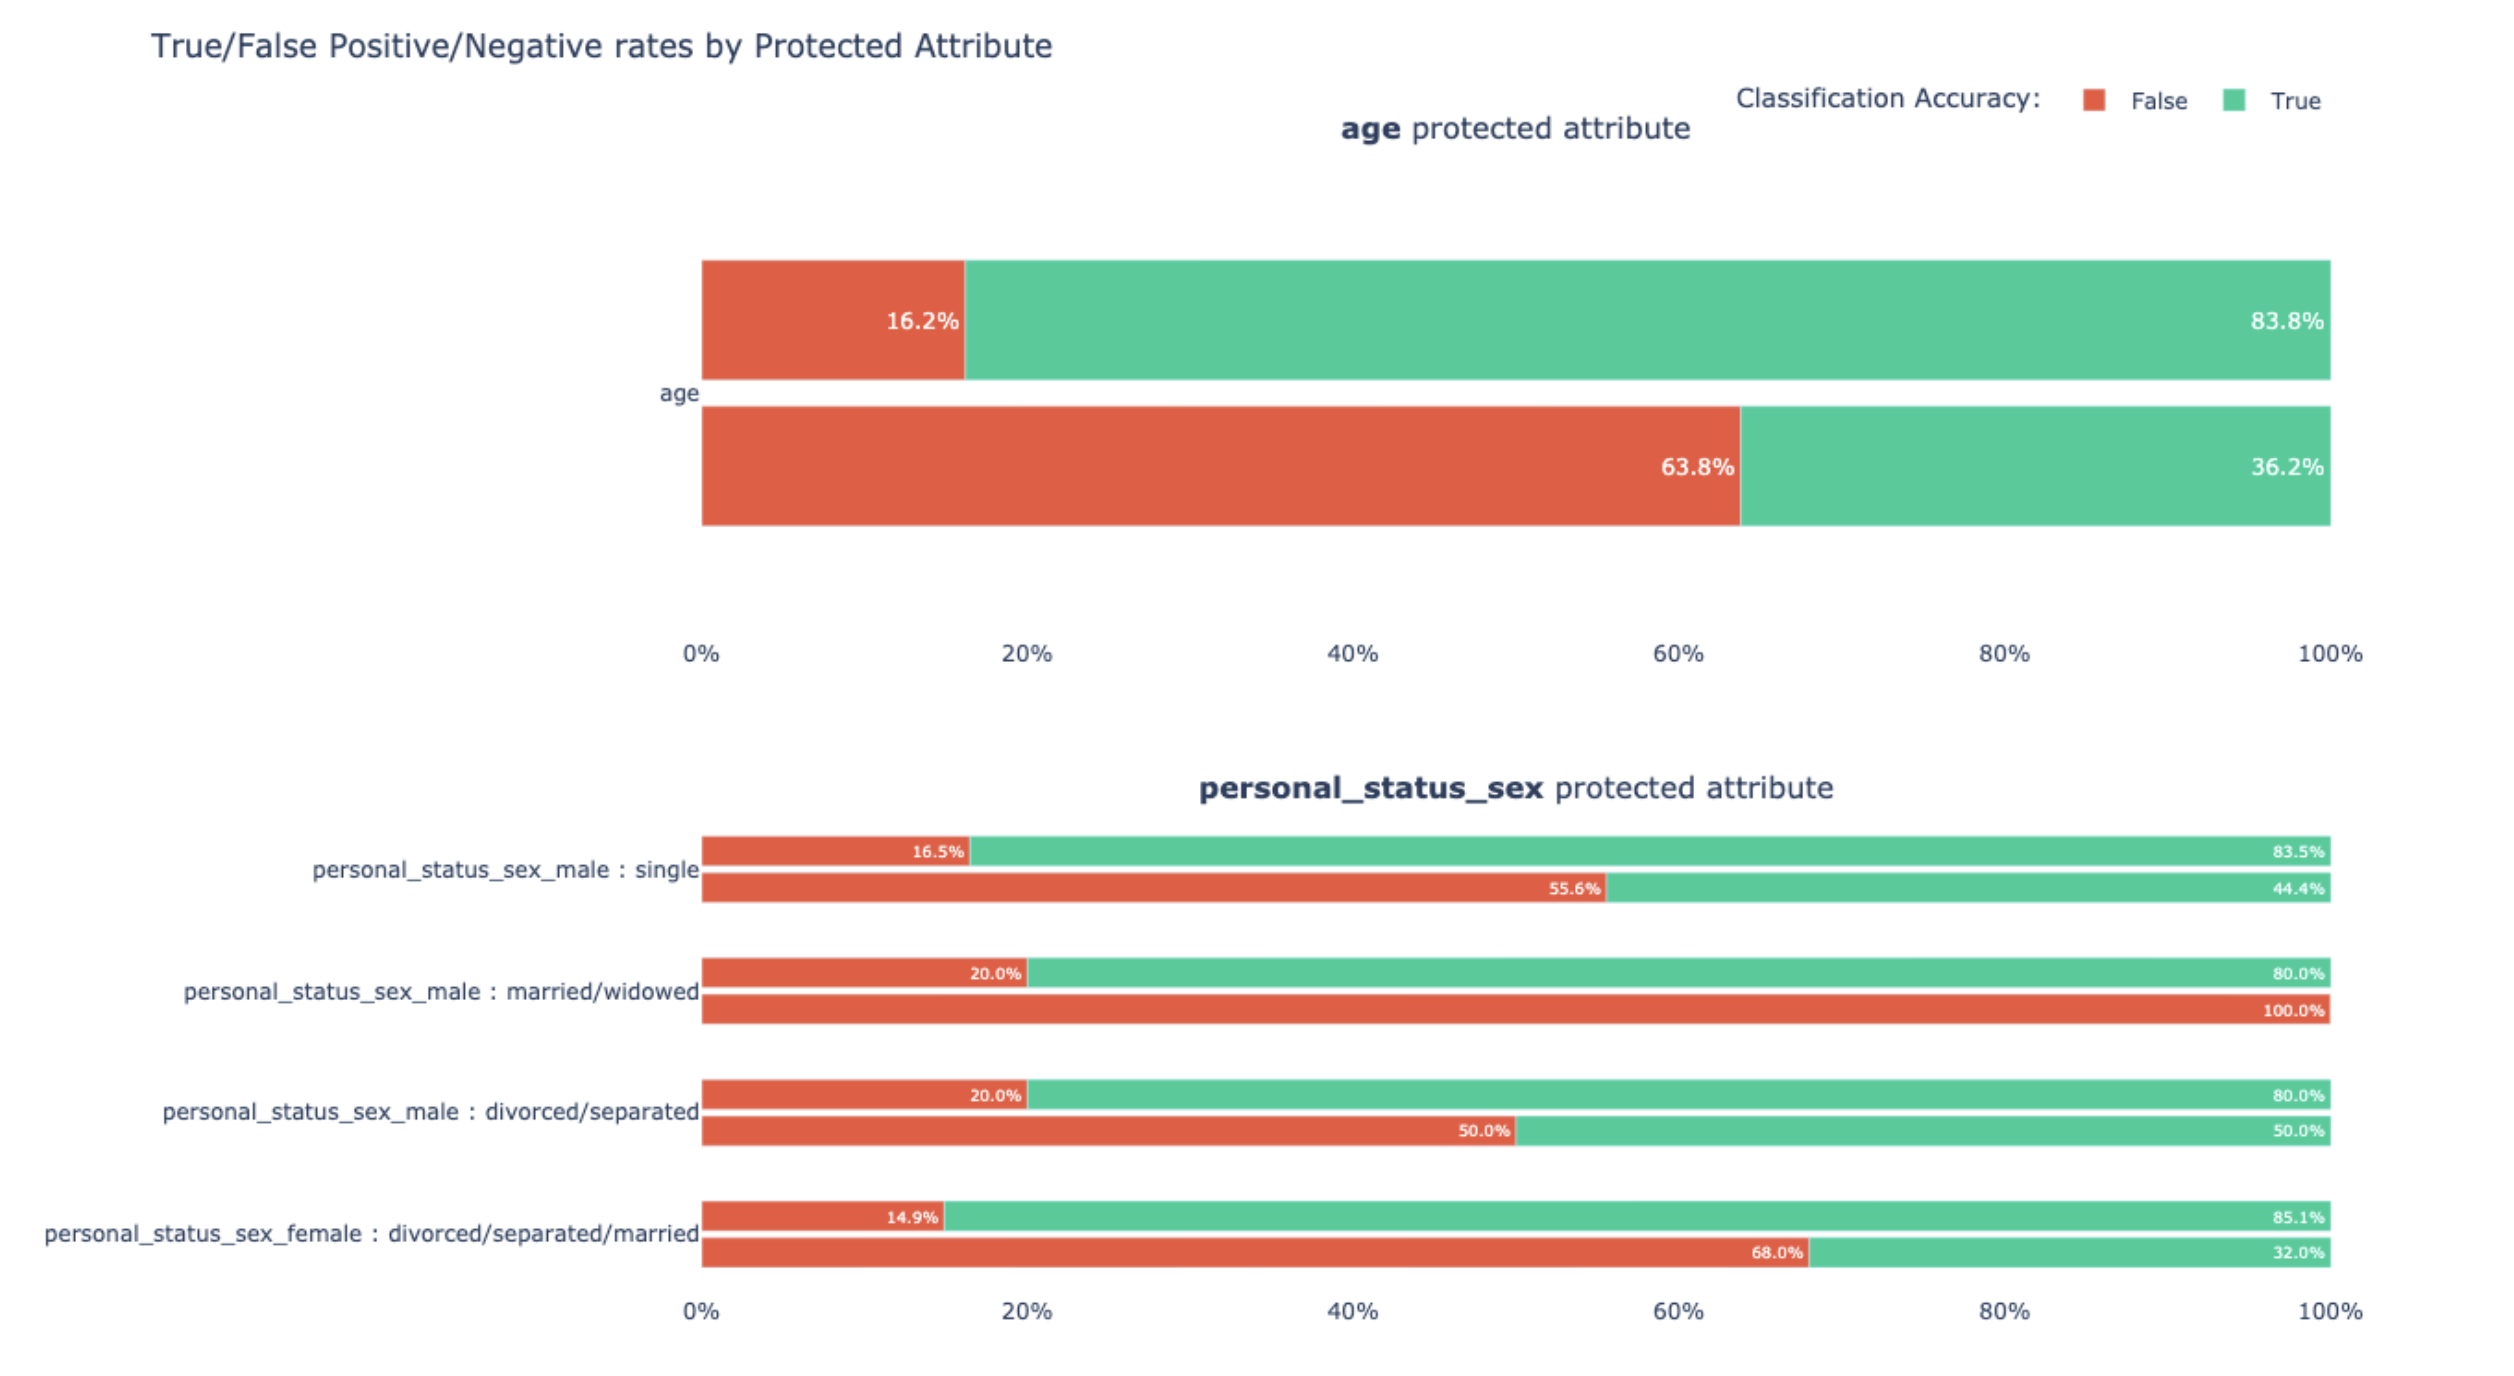
\includegraphics[width=0.89\textwidth]{images/true-false-outcomes.png}
\caption{True/False Positive/Negative rates by protected attribute(s)} \label{true-false-outcomes}
\end{figure}

\subsection{MinDiff}
The MinDiff regularization technique aims to minimize the difference in prediction scores between groups defined by a sensitive attribute. This approach directly addresses disparities by forcing the model to make more similar predictions for individuals who are similar in all respects except for their protected attributes.

\begin{equation}
\mathrm{MinDiff} = \left| P(\hat{Y} = 1 \mid A = a) - P(\hat{Y} = 1 \mid A = b) \right|
\end{equation}

Depending on the specific implementation and the nature of the data, MinDiff can be visualized in various ways. One approach is to show the distribution of prediction scores for different groups before and after applying MinDiff. This allows users to see how the technique reduces the gap in prediction scores between groups. In our current solution, we do not utilize with visualization the MinDiff method yet.

\subsection{Correlations to the prediction outcome}
Determining any biases and dependencies in the data requires an understanding of the relationship between features and the model's anticipated result. The degree to which various variables dramatically affect predictions—whether in a favorable or negative way—is shown by correlation analysis. While a near-zero correlation suggests little to no direct impact, a high correlation indicates a substantial association between the trait and the expected outcome.\\

Two correlation heatmaps are used to illustrate this. A comprehensive picture of the relationship between many attributes and the prediction result is provided by the first heatmap, which shows the correlation values for every attribute. The second heatmap highlights the particular impact of the chosen protected attribute on predictions, concentrating strictly on that.

\begin{figure}[H]
\centering
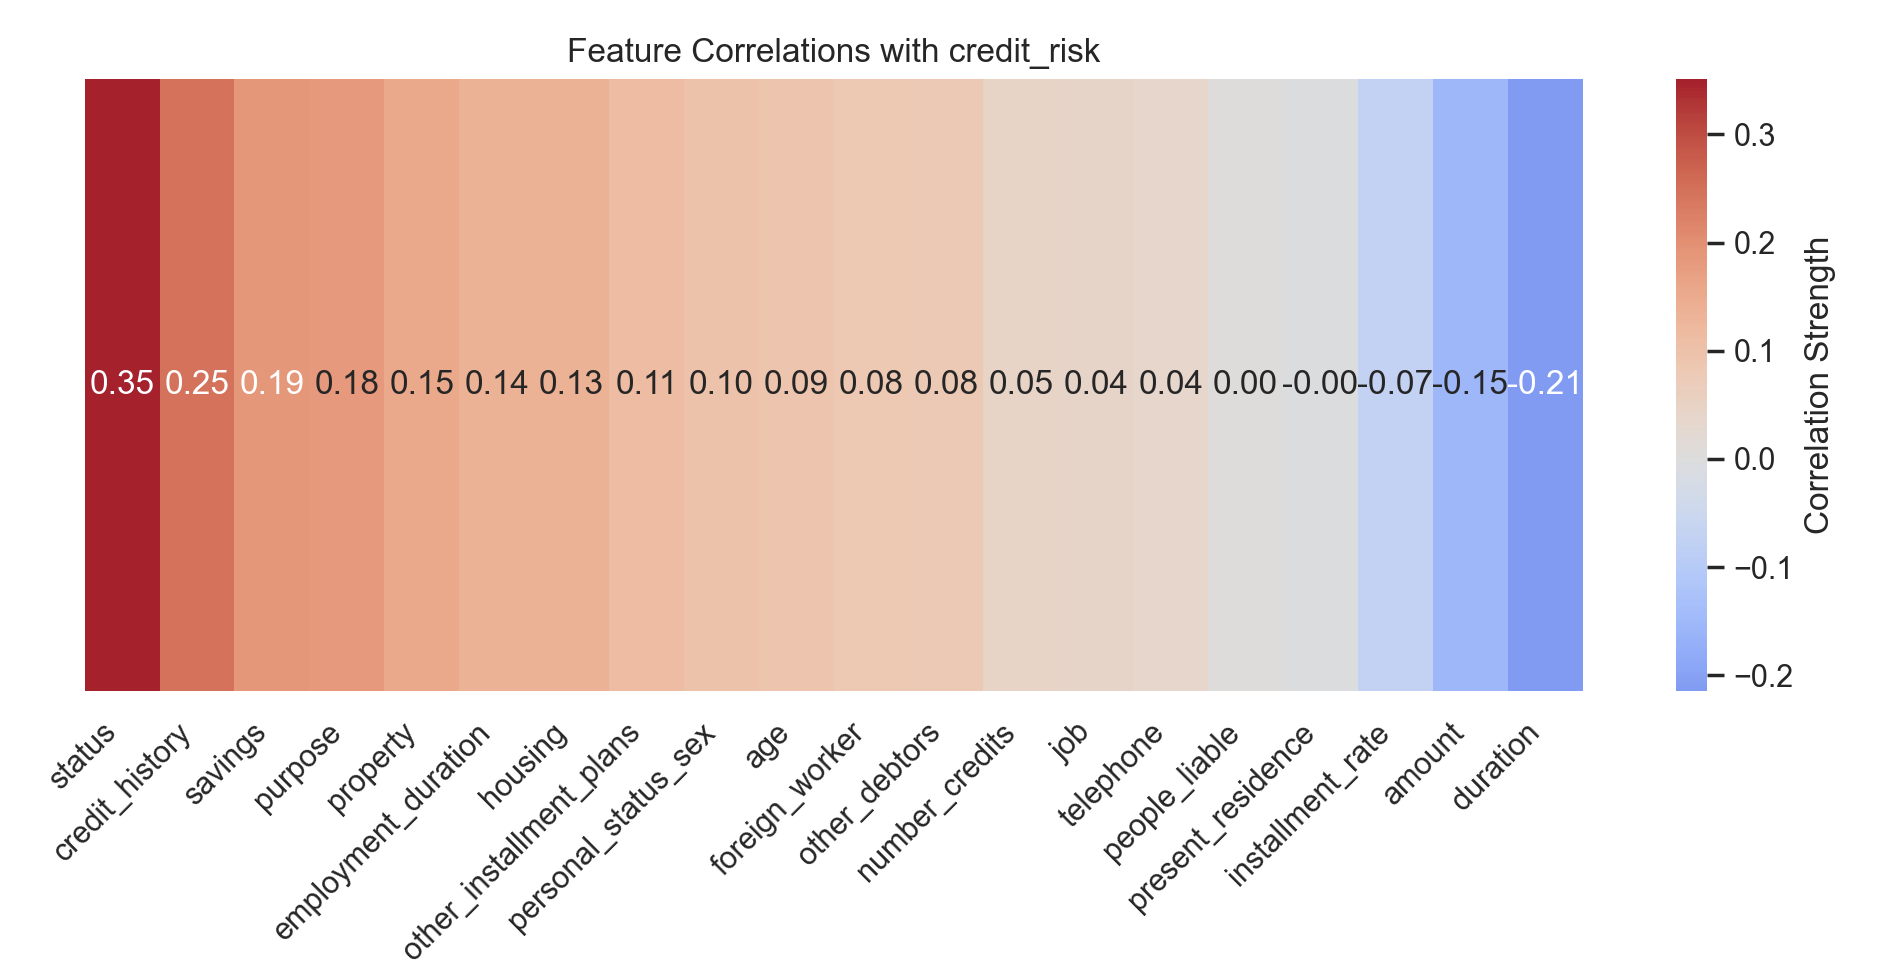
\includegraphics[width=0.7\textwidth]{images/feature-correlation.png}
\caption{Correlations of all attributes to predicted feature} \label{cfeature-correlation}
\end{figure}

\begin{figure}[H]
\centering
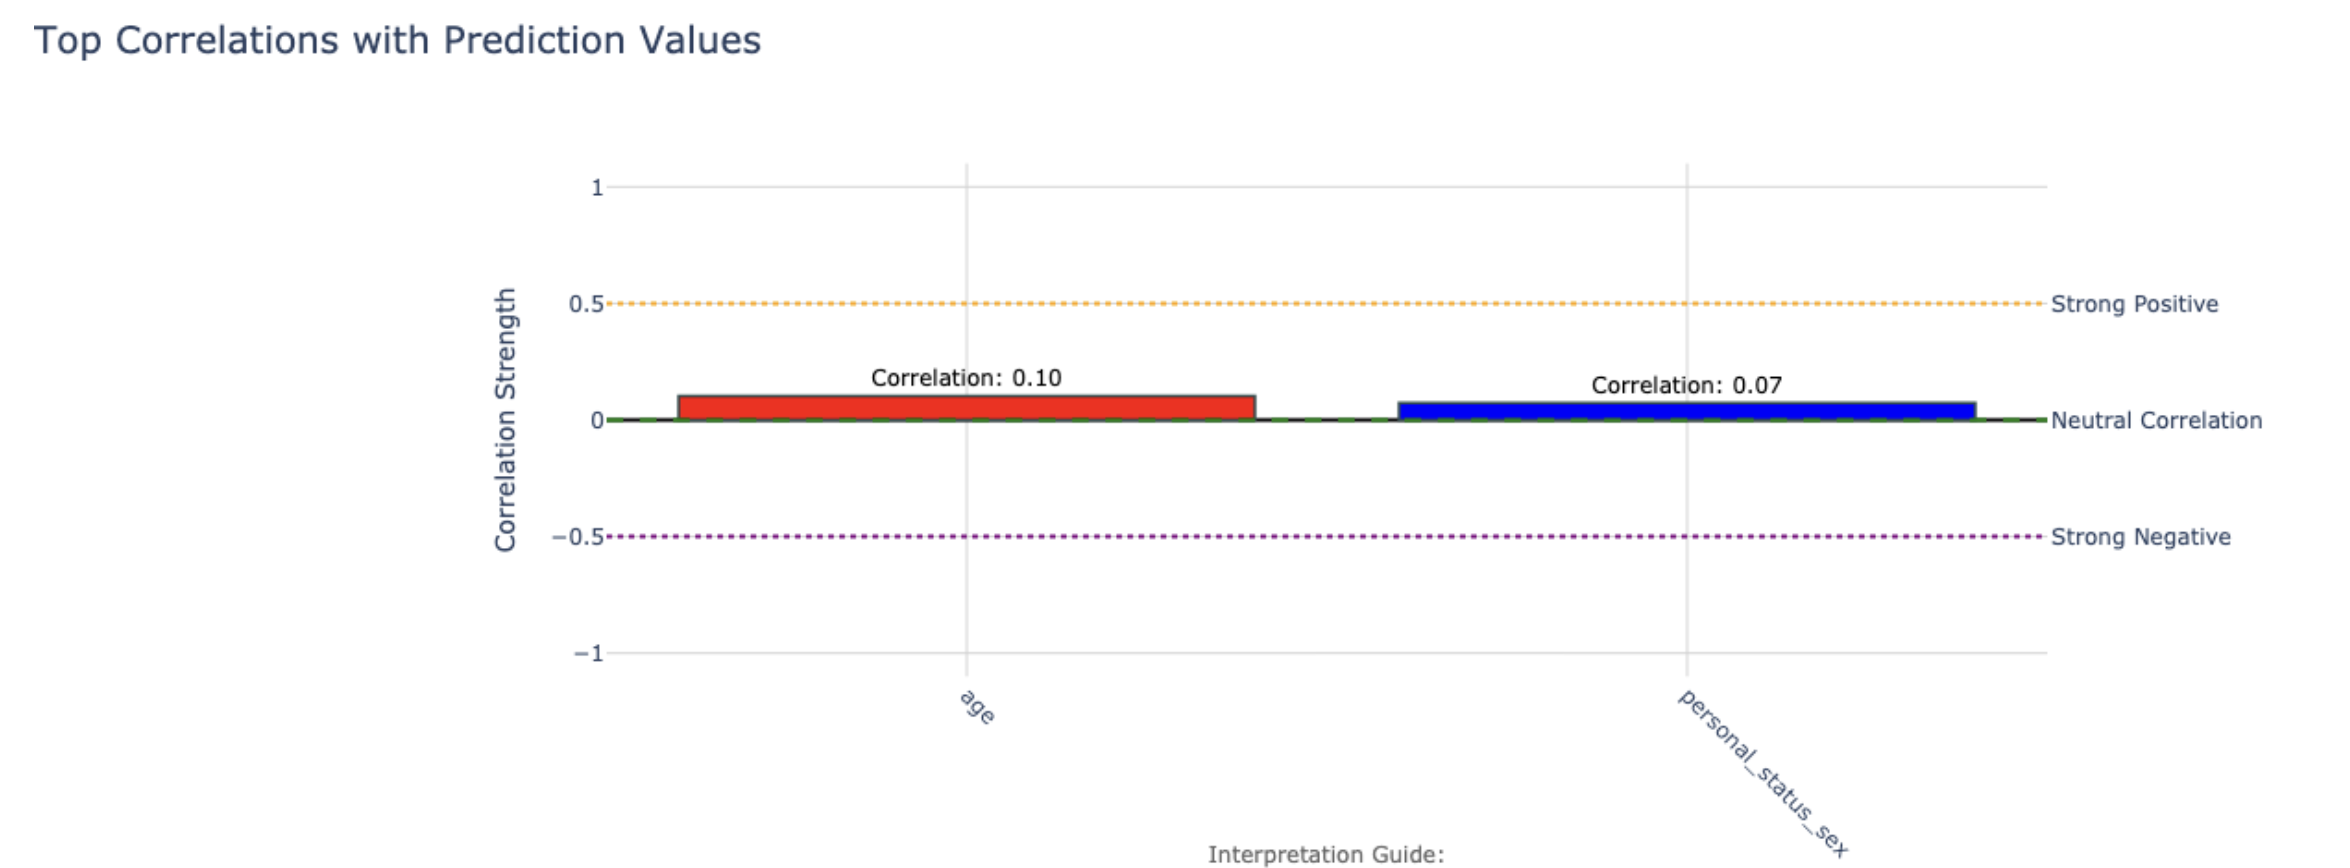
\includegraphics[width=0.9\textwidth]{images/correlation-chart.png}
\caption{Correlations of the chosen protected attribute(s) to predicted feature} \label{correlation-chart}
\end{figure}

A higher feature value is correlated with a higher number of positive predictions in these visualizations, where red denotes stronger correlations and deeper shades indicate a stronger positive link. On the other hand, blue denotes stronger negative correlations, where a lesser chance of a good prediction is linked to a higher feature value. With values close to zero, neutral correlations show that there is little to no linear relationship between the feature and the forecast result.

\section{Experiments and Result}
\subsection{Improvement from State-of-the-Art}
Our solution, \href{https://github.com/bence749/fairnessLens}{FairnessLens} distinguishes itself from existing state-of-the-art tools like AIF360 and Fairlearn – tools which, as the literature suggests, can present visualizations that are "too comprehensive" for non-technical users – in several key aspects.\\

\begin{figure}[H]
\centering

\includegraphics[width=0.5\textwidth]{images/fairnesslens-logo.png}
\caption{FairnessLens logo} \label{fairnesslens-logo}
\end{figure}

By leveraging Jupyter Notebook and Mercury, we provide a more intuitive and interactive user experience, particularly for users without extensive technical expertise. The simple dataset upload and (protected) attribute selection process lowers the barrier to entry for fairness assessment. This directly addresses the recurring issue of "the absence of tools designed to foster intuitive understanding rather than relying solely on mathematical representations," highlighted by Chouldechova ~\cite{chouldechova2017}.\\

Our tool goes beyond simply reporting fairness metrics. We provide users with clear, actionable guidance on how to mitigate identified biases, including recommendations on appropriate pre-processing and post-processing techniques.\\

We integrate visualizations directly with metric calculations and model training results, enabling users to easily explore the impact of different fairness interventions. Furthermore, we aim to incorporate explainability techniques to provide insights into why certain biases exist and how they can be addressed. This addresses the need for "interpretability and explainability" which are increasingly becoming crucial elements of fairness research.

\begin{figure}
\centering
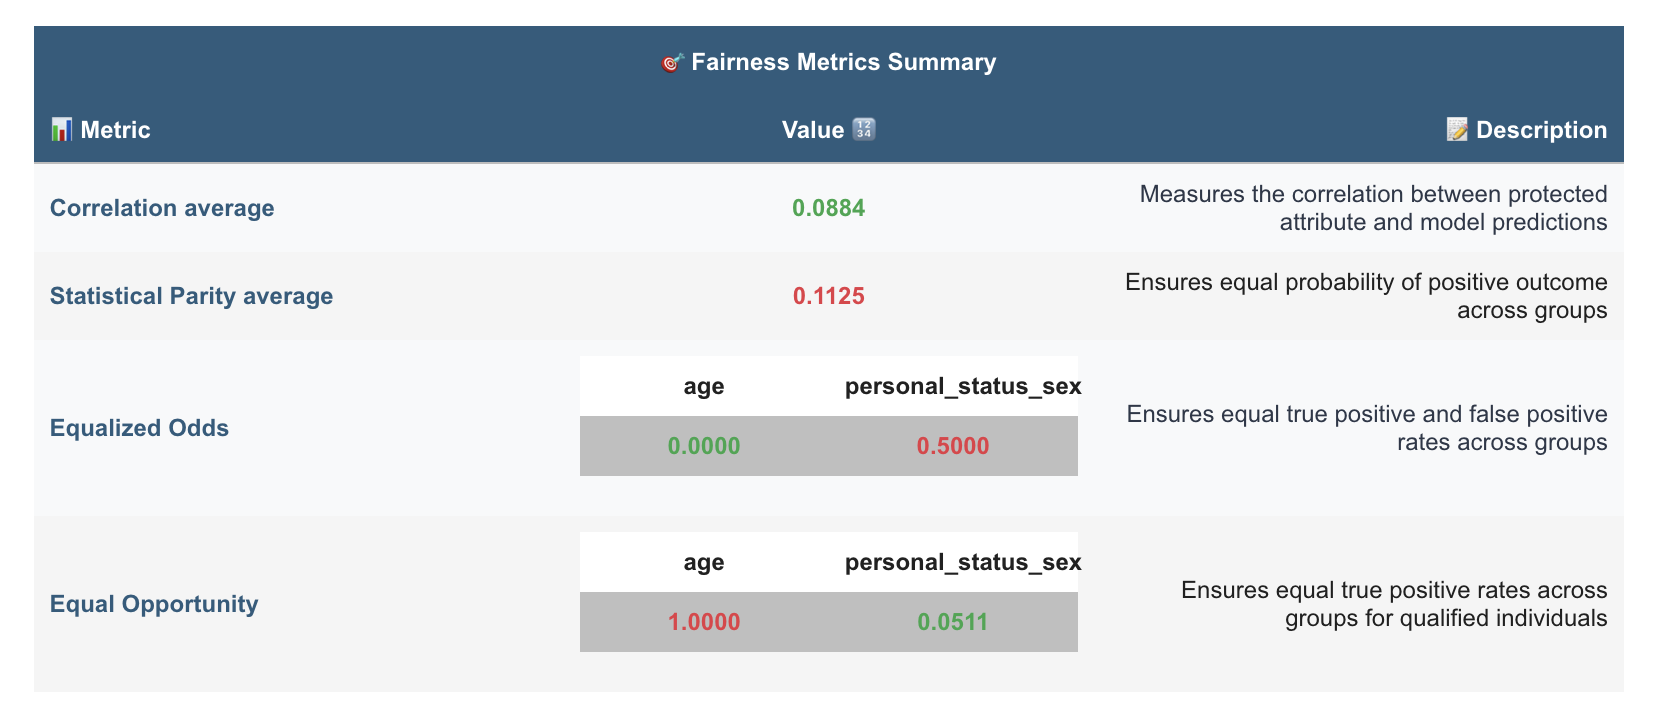
\includegraphics[width=1\textwidth]{images/fairness-metrics-summary.png}
\caption{Fairness Metrics Summary} \label{fairness-metrics-summary}
\end{figure}

We emphasize the importance of justifying fairness interventions by providing users with tools to document the rationale behind their decisions and the trade-offs involved. This supports transparency and accountability in the development of fair ML models.

\section{Discussion}
This scientific research aims to provide a practical and accessible solution to the identified challenges\cite{caton2024fairness} in achieving fairness in machine learning models, moving beyond theoretical discussions to offer a tangible tool for practitioners. Our approach focuses on creating interactive visualizations and actionable guidance, addressing the gap between intricate technical principles and practical understanding.

\subsection{Interpretation of Results}
The results of our experiments, as detailed in Section 6, are expected to demonstrate the effectiveness of our fairness assessment tool in empowering users to identify and mitigate biases in their datasets and models. We anticipate that the accuracy of metric calculations will closely align with those of established fairness libraries like AIF360 and Fairlearn, validating the reliability of our tool's core computations. Furthermore, we expect the usability studies to indicate that our tool is user-friendly and accessible, even for individuals with limited technical expertise. User surveys and interviews will be used to evaluate the efficacy of our visualizations, and we hope to receive good feedback on the tool's capacity to communicate fairness and bias in an  understandable and straightforward way.

\subsection{Implications of Findings}
Our findings have several important implications for the field of fairness in machine learning. First, they demonstrate the value of interactive visualizations and actionable guidance in making fairness assessment more accessible to a wider audience. By providing users with intuitive tools and clear recommendations and documentation, we empower them to take concrete steps to address biases and promote fairness in their models. Second, our research highlights the importance of considering trade-offs between fairness and other performance goals, such as accuracy. As discussed in Section 3, achieving fairness often involves making compromises and it is essential to carefully consider the implications of these trade-offs in the context of specific applications. Finally, our work contributes to the ongoing effort to develop more comprehensive and user-friendly tools for fairness assessment, addressing a key need identified in the state-of-the-art.

\subsection{Limitations and Future Work}
Despite the anticipated positive results, our research has several limitations that should be acknowledged. First, our evaluation is limited to the specific datasets and metrics used in our experiments. Future work should explore the tool's performance across a wider range of datasets and fairness metrics, including individual fairness measures and intersectional fairness concerns. Second, our tool currently focuses on a specific set of pre-processing and post-processing techniques. Future work could explore the integration of additional mitigation strategies, including causal fairness approaches and fairness-aware AutoML.\\

On top of that, our current work is focused on classification models. Future efforts should explore extending the tool to other model types, such as regression, to support a wider range of machine learning applications.
Finally, our research has not yet addressed the challenge of justifying fairness interventions and documenting trade-offs. Future work should focus on developing more robust mechanisms for supporting this critical aspect of fairness assessment.

\section{Conclusion and Summary}
This research has presented a fresh approach to addressing the challenges of fairness in ML, focusing on the development and evaluation of a user-friendly and accessible fairness assessment tool. By leveraging interactive visualizations and actionable guidance, our work aimed to bridge the gap between intricate technical principles and practical understanding, enabling both technical and non-technical users to actively engage with and mitigate biases in their AI systems. This aligns directly with the urgent demand identified in the literature for better visualization methods – tools that are user-friendly and efficient in conveying insights linked to fairness. As noted in our state-of-the-art review, the field can close the gap between technical complexity and practical understanding by concentrating on developing more approachable, interactive and example-driven visualization techniques, guaranteeing that fairness becomes an understandable and achievable objective for all parties involved. Our work seeks to directly address this need.

\subsection{Key Contributions}
The key contributions of our research build upon existing tools and frameworks for fairness, addressing their identified limitations and going beyond heatmaps. Our work has produced concrete outcomes:\\

The development of FairnesLens provides an intuitive interface for uploading data, selecting attributes, calculating fairness metrics and visualizing results. As opposed to current solutions that may be too complicated for non-technical users, its interactive nature encourages users to explore different fairness interventions and understand their impact on model performance easily.\\

In the production of a \textit{Comprehensive Evaluation Framework}, we designed and implemented a rigorous evaluation framework to assess the effectiveness of our tool across a diverse set of datasets and fairness metrics. Our results show that the tool can assist users in successfully spotting and lessening biases in their models, showing its usefulness in real-world circumstances.\\

With the focus on \textit{Actionable Guidance and Recommendation}, our tool goes beyond just providing fairness indicators by giving users explicit, doable guidance on how to reduce identified biases and a way to justify fairness measures and record trade-offs. By addressing the necessity for understandable justifications and encouraging transparency in fairness interventions, this characteristic supports responsible AI development.\\

In the response on \textit{Addressing a Critical Need}, our tool directly addresses the critical need for more interactive, intuitive, and instructional visualization techniques, as highlighted in the state-of-the-art. Unlike existing bias heatmaps and disparity matrices that require careful interpretation, our tool aims to provide visualizations that are easily understandable by both technical and non-technical users.

\subsection{Future Improvements}
While our research has made significant progress in addressing the challenges of fairness in machine learning, several opportunities exist for future improvements. These include:\\

As fairness research progresses, new and more nuanced metrics are being developed, future versions of our tool could incorporate a wider range of these, including individual fairness measures, intersectional fairness concerns and causal fairness measures, to provide a more comprehensive assessment of fairness.\\

Our tool currently focuses on a specific set of pre-processing and post-processing techniques. Future work could explore integrating additional mitigation strategies, including fairness-aware AutoML and reinforcement learning-based fairness interventions, to provide users with a broader range of options for mitigating bias.\\

While our tool provides actionable guidance for mitigating biases, it could be further enhanced by incorporating explainability techniques to help users understand why certain interventions work and how they affect different subgroups of the population. This could involve integrating SHAP values or other explainability methods into the visualizations to provide deeper insights into the model's behavior.\\

Finally, the true test of our tool's effectiveness will come from its deployment in real-world settings. Future work should focus on deploying the tool in various practical applications and conducting user studies to assess its impact on the development and deployment of fair AI systems.

\subsection{Final Remarks}
In conclusion, our research has presented a practical and accessible solution to the challenges of fairness assessment in machine learning. By providing users with a user-friendly tool, a comprehensive evaluation framework and actionable guidance, we hope to empower them to build more equitable and transparent AI systems. While much work remains, we believe our research represents a significant step forward in the pursuit of fairness in AI. As hybrid approaches that include pre- and post-processing techniques become more popular, our tool will be essential in offering actionable items and insights. It will empower everyone to follow the path and have more reliable and responsible results. Further investigation is still needed for improvements in the future, but the journey towards fairer and more ethical AI has taken a positive step.
%
% ---- Bibliography ----
%
% BibTeX users should specify bibliography style 'splncs04'.
% References will then be sorted and formatted in the correct style.
%
% \bibliographystyle{splncs04}
% \bibliography{mybibliography}
%
\begin{thebibliography}{8}
\bibitem{dibello2021fairness}
Di Bello, M.: Algorithmic Fairness: Structural Perspectives. Available at \url{https://www.marcellodibello.com/algorithmicfairness/handout/structural.html} (2021).

\bibitem{fraenkel2020fairness}
Fraenkel, A.: Fairness \& Algorithmic Decision Making. Self-Published, Available at \url{https://afraenkel.github.io/fairness-book/content/05-parity-measures.html} (2020).

\bibitem{bell2023fairness}
Bell, A., Bynum, L., Drushchak, N., Zakharchenko, T., Rosenblatt, L., Stoyanovich, J.: The Possibility of Fairness: Revisiting the Impossibility Theorem in Practice. Proceedings of the ACM Conference, Available at \url{https://dl.acm.org/doi/abs/10.1145/3593013.3594007} (2023).

\bibitem{nguyen2022fairness}
Nguyen, M.: Poster: The Impossible Theorem of Fairness. Available at \url{https://digitalcommons.hamilton.edu/cgi/viewcontent.cgi?article=1006} (2022).

\bibitem{kleinberg2016}
Kleinberg, J., Mullainathan, S., Raghavan, M.: Inherent Trade-Offs in the Fair Determination of Risk Scores. ArXiv, Available at \url{https://arxiv.org/abs/1609.05807} (2016). Accessed: 2025-02-24.

\bibitem{yap2024}
Yap, J.Q., Lim, E.: A legal framework for artificial intelligence fairness reporting. The Cambridge Law Journal, Available at \url{https://www.cambridge.org/legal-framework-for-artificial-intelligence-fairness-reporting} (2024).

\bibitem{prince2019}
Prince, S.: Tutorial \#1: Bias and fairness in AI. Available at \url{https://rbcborealis.com/research-blogs/tutorial1-bias-and-fairness-ai} (2019). Accessed: 2025-02-24.

\bibitem{voria2024}
Voria, G., Sellitto, G., Ferrara, C., Abate, F., De Lucia, A., Ferrucci, F., Catolino, G., Palomba, F.: A Catalog of Fairness-Aware Practices in Machine Learning Engineering. ArXiv, Available at \url{https://arxiv.org/abs/2408.16683} (2024). Accessed: 2025-02-24.

\bibitem{hardt2016}
Hardt, M., Price, E., Srebro, N.: Equality of Opportunity in Supervised Learning. ArXiv, Available at \url{https://arxiv.org/abs/1610.02413} (2016). Accessed: 2025-02-24.

\bibitem{google2024bias}
Google LLC: Addressing Bias and Fairness Issues in ML Models. Available at \url{https://colab.research.google.com/github/google/eng-edu/blob/main/ml/cc/exercises/fairness_income.ipynb} (2024).

\bibitem{precioso2024ethical}
Precioso, F.: SI5 – IA-ID Advanced Deep Learning 2024-2025: Ethical Aspects of Data Fairness, Bias, Mitigation. (2024).

\bibitem{bengio2024}
Bengio, Y.: International Scientific Report on the Safety of Advanced AI. Available at \url{https://www.gov.uk/government/publications/international-scientific-report-on-the-safety-of-advanced-ai} (2024). Accessed: 2025-02-24.

\bibitem{mbakwe2023}
Mbakwe, A.B., Lourentzou, I., Celi, L.A., Wu, J.T.: Fairness metrics for health AI: we have a long way to go. Available at \url{https://pmc.ncbi.nlm.nih.gov/articles/PMC10114188} (2023). Accessed: 2025-02-24.

\bibitem{zohar2023}
Zohar, Y.: Fairness Metrics in Machine Learning. Available at \url{https://www.marcellodibello.com/algorithmicfairness/handout/impossibility.html} (2023). Accessed: 2025-02-24.

\bibitem{chouldechova2017}
Chouldechova, A.: Fair prediction with disparate impact: A study of bias in recidivism prediction instruments. In: Proceedings of the 2017 ACM Conference on Fairness, Accountability, and Transparency, pp. 1--13 (2017). \doi{10.48550/arXiv.1703.00056}.

\bibitem{caton2024fairness}
Caton, S., Haas, C.: Fairness in Machine Learning: A Survey. ACM Comput. Surv. 56, 7, Article 166 (July 2024), 38 pages. Available at \url{https://doi.org/10.1145/3616865} (2024).

\end{thebibliography}
\appendix

\section{Annex}
\subsection{Software Delivery Sheet} 
Signatures are redacted for privacy reasons. This is a publicly available research paper.
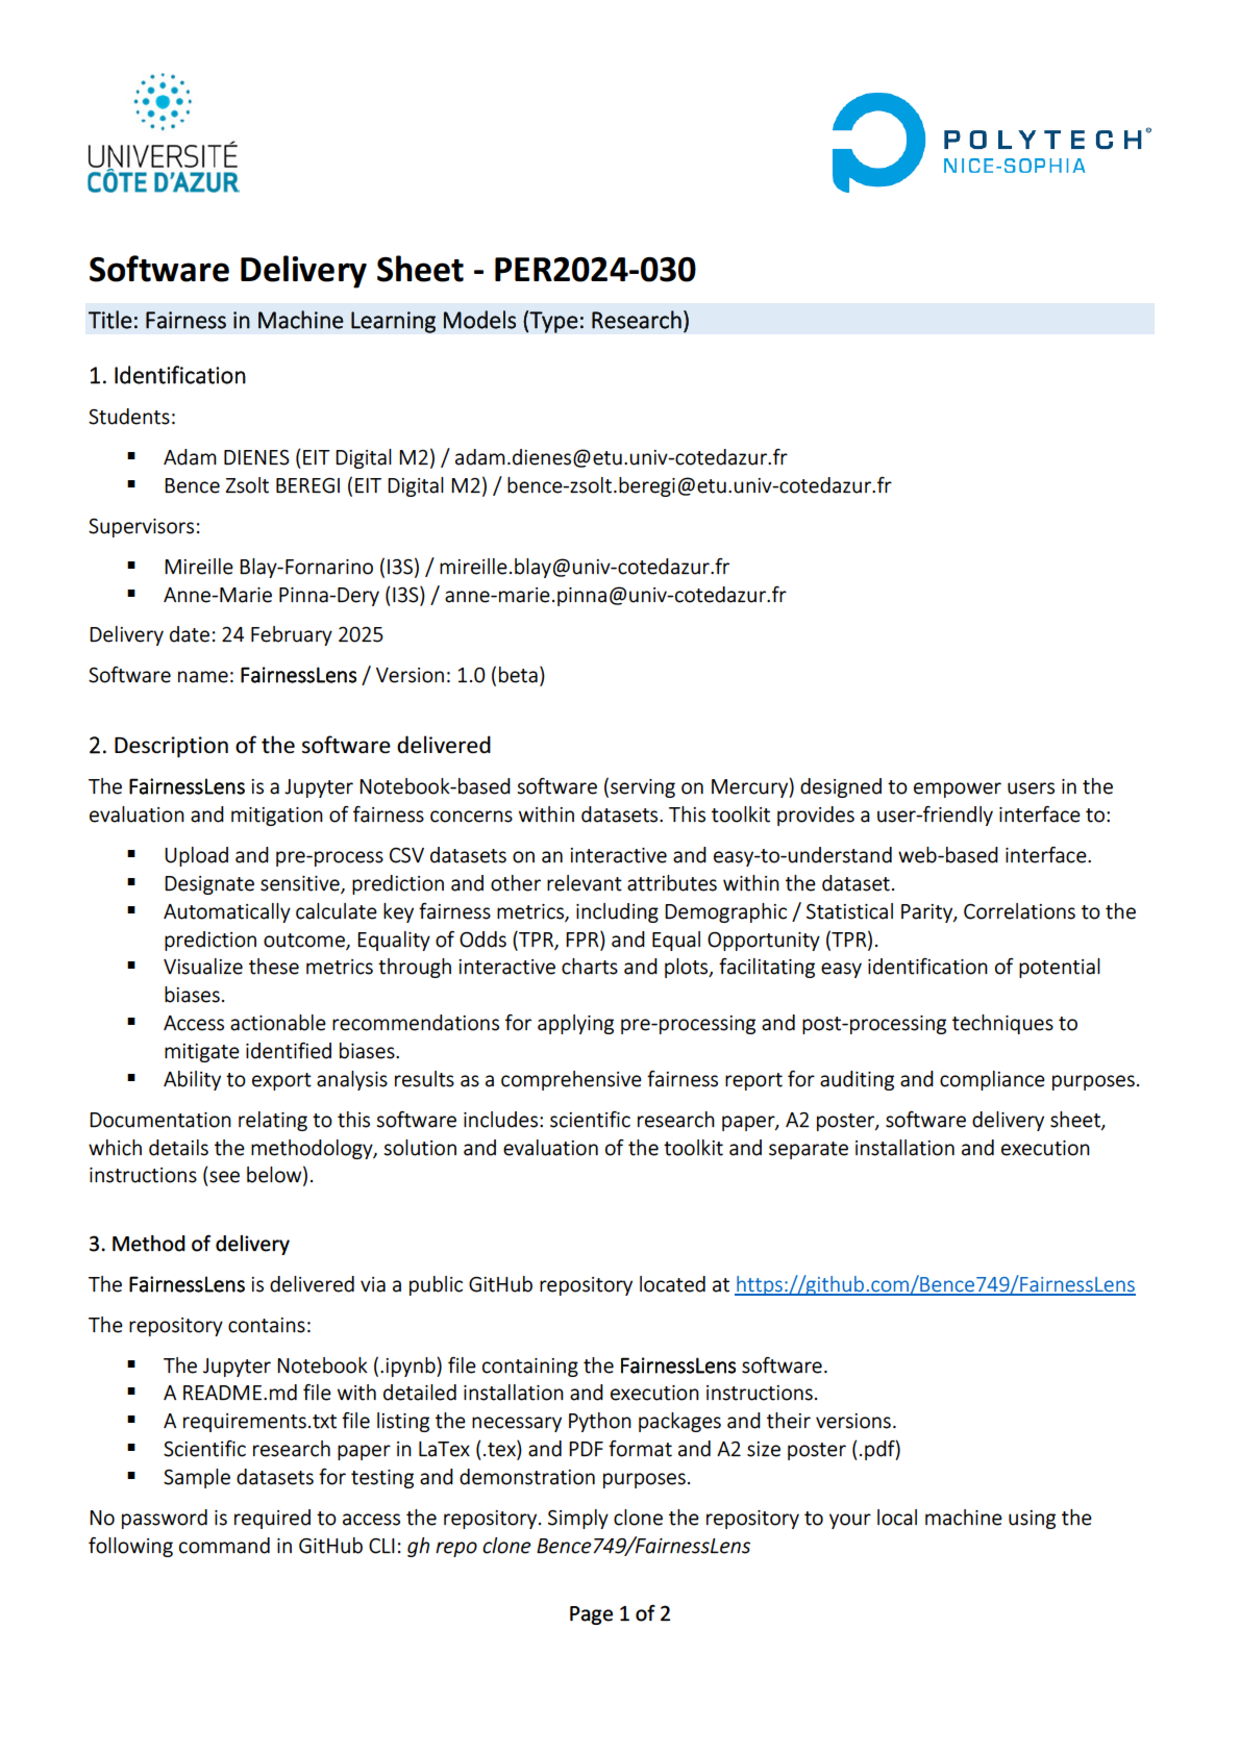
\includepdf[pages=-]{embed/software-delivery-sheet-redacted.pdf}
\end{document}
